\documentclass[12pt]{article}
\usepackage[margin=1in]{geometry}
\usepackage{amsmath, amsthm, amssymb, amsfonts, breqn, graphicx}


\theoremstyle{definition}
\newtheorem{problem}{Problem}
\renewcommand*{\proofname}{Solution}
\newenvironment{custompbm}[1]
  {\renewcommand\theproblem{#1}\problem}
  {\endproblem}
\renewcommand{\theenumi}{\alph{enumi}}


\newcommand{\E}{\text{E}}
\newcommand{\V}{\text{Var}}
\newcommand{\Co}[2]{\text{Cov}\left({#1}, {#2}\right)}
\newcommand{\pdf}{\text{pdf}}
\newcommand{\pmf}{\text{pmf}}
\newcommand{\me}{\mathrm{e}}
\newcommand*\diff{\mathop{}\!\mathrm{d}}
\newcommand{\vect}[1]{\boldsymbol{#1}}
\newcommand{\mx}[1][t]{\mu_X({#1})}
\newcommand{\gx}[2]{\gamma_X({#1}, {#2})}


\title{Homework Assignment 10}
\author{Matthew Tiger}


\begin{document}


\maketitle


\begin{problem}
  Plot the energy bills versus time. What kind of trend appears to exist? What type of seasonal
  variation appears to exist? Is a transformation needed to obtain a series that displays constant
  variation?
\end{problem}

\begin{proof}
  See below for a plot of the bills time series data:
  \vskip 0mm
  \begin{center}
  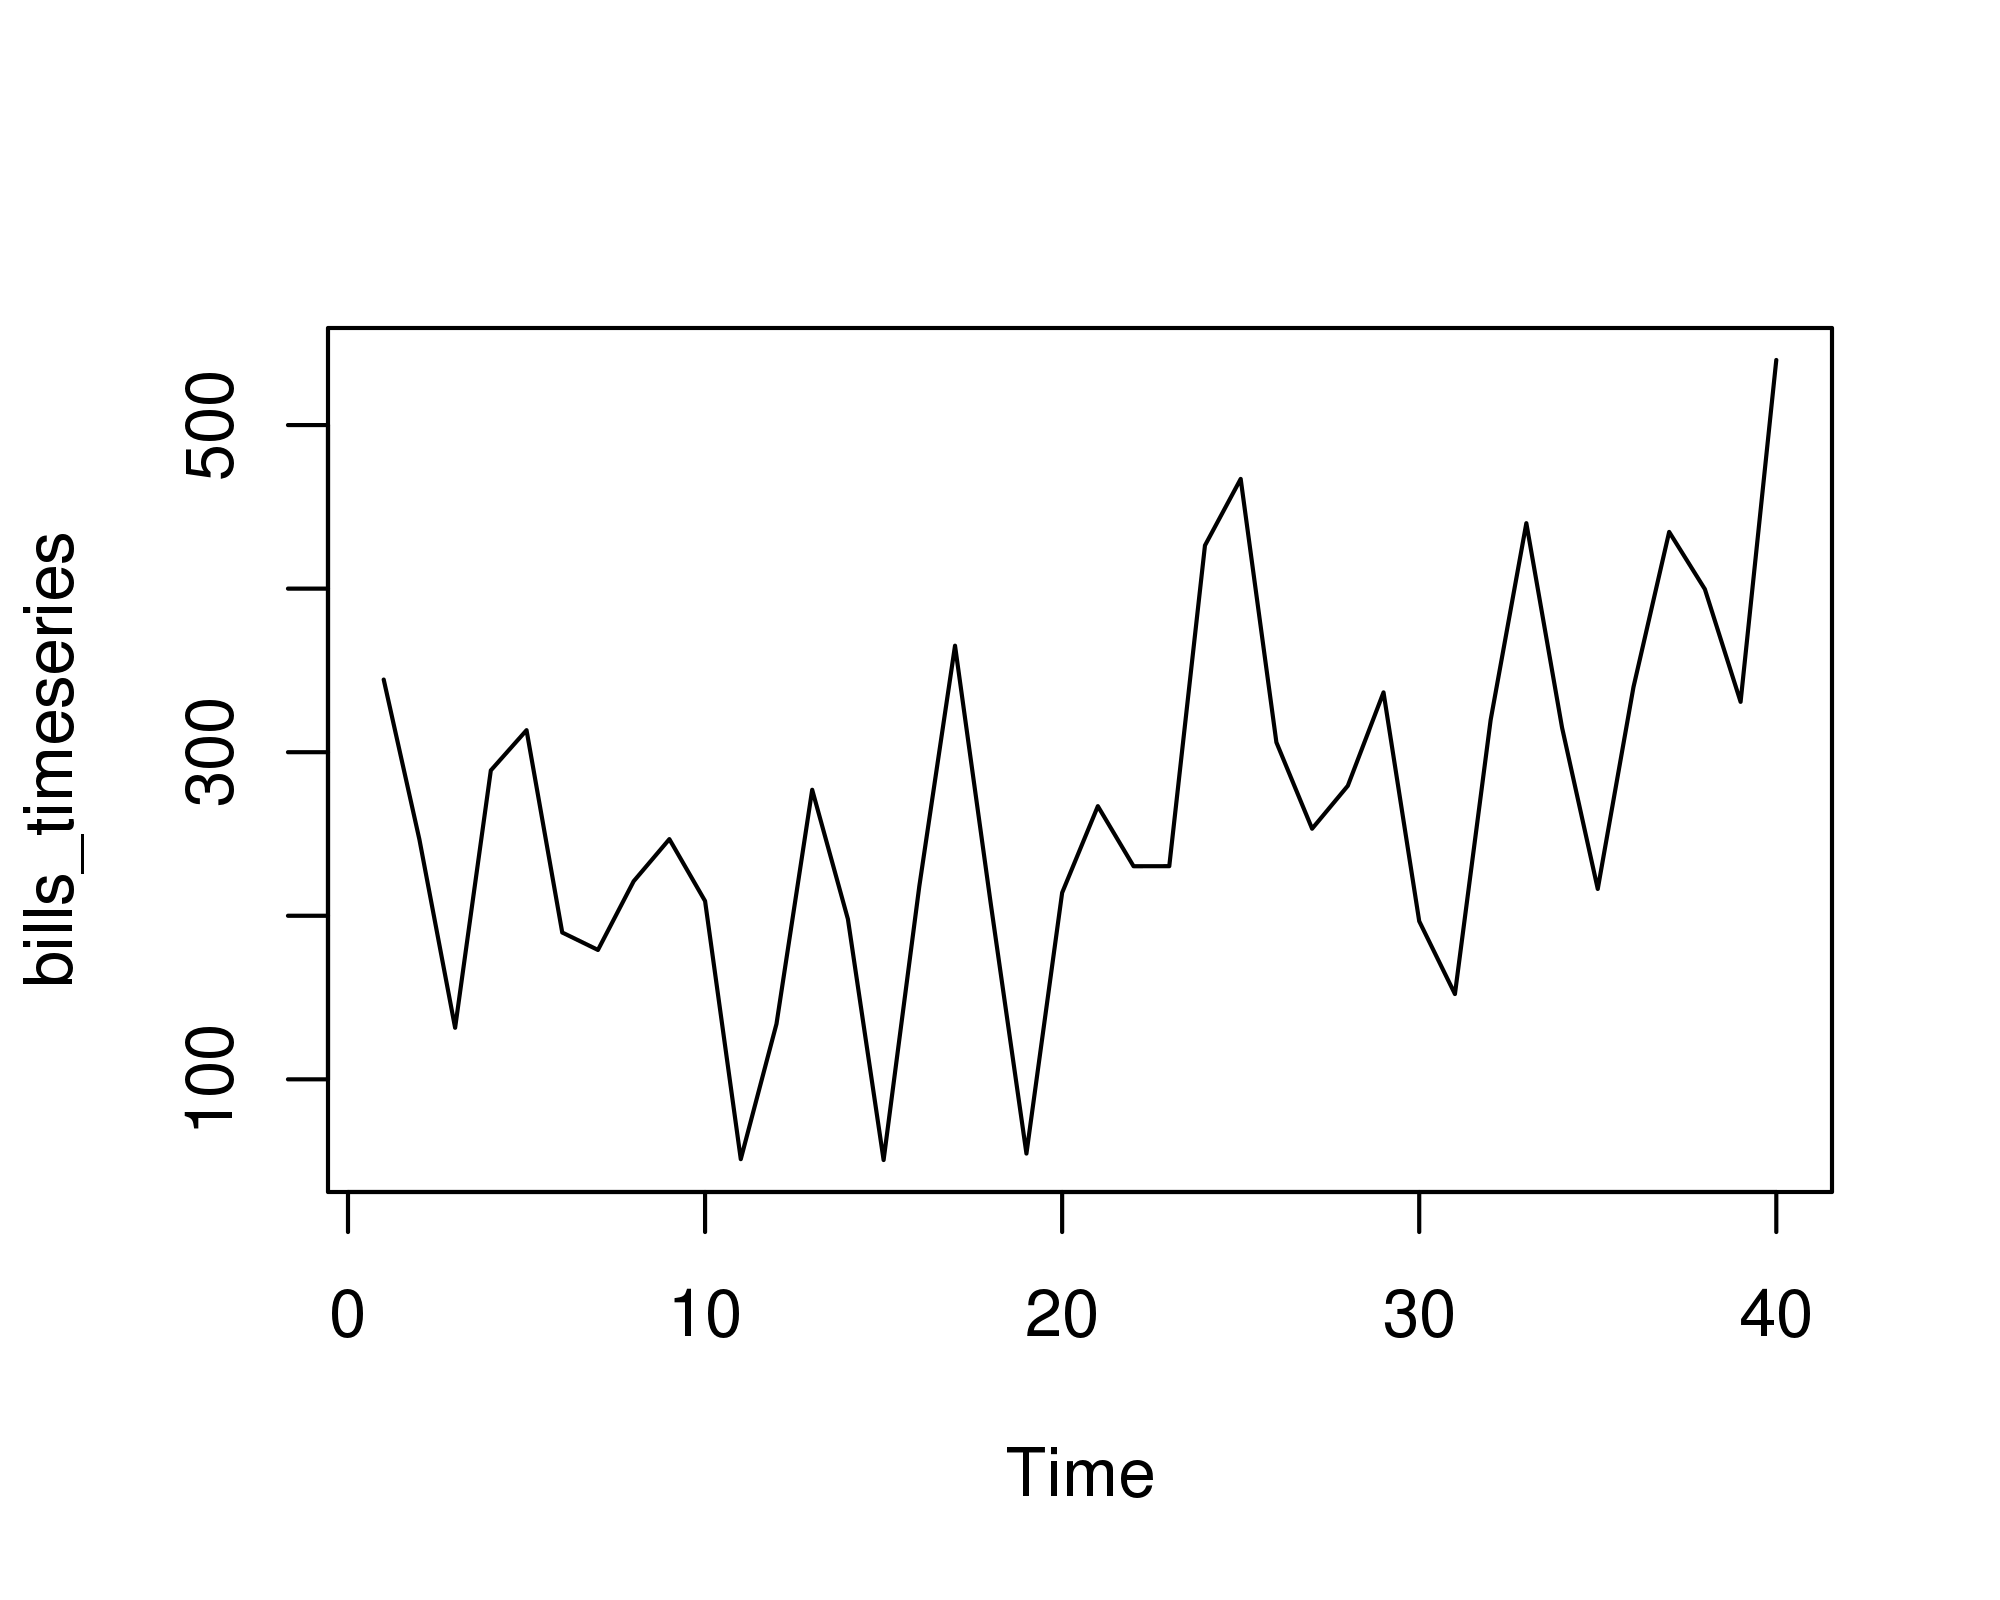
\includegraphics{timeseries}
  \end{center}
  \vskip 10mm

  It is clear from the plot that there is a trend that appears to move upwards
  as time increases and a seasonal variation with period 4
  lags present in the data so a transformation is needed to obtain residuals
  that represent a stationary time series.
\end{proof}


\begin{problem}
  Write algebraically a time series model with trend and seasonal component with definitions
  of the dummy variable.
\end{problem}

\begin{proof}
  Note that it appears that this time series has a quadratic trend. Additionally,
  we are interested in capturing the seasonal quarter data of the time series.
  Therefore, a time series model for the data with trend and seasonal components is given by
  \[
    X_t = a_0 + a_1 t + a_2 t^2 + a_3 Q_1 + a_4 Q_2 + a_5 Q_3 + a_6 Q_4,
  \]
  where we define $Q_i$ as 1 if $t \equiv i \mod 4$ and 0 otherwise and $a_j$ is
  constant.
\end{proof}

\end{document}
